\title{Data Mining - Aufgabenblatt 3}
\author{Andra Herta, Tobias Dreher}
\date{19.12.2011}

\documentclass[%
	pdftex,%              PDFTex verwenden da wir ausschliesslich ein PDF erzeugen.
	oneside,%             Einseitiger Druck.
	12pt,%                Grosse Schrift, besser geeignet für A4.
	parskip=half,%        Halbe Zeile Abstand zwischen Absätzen.
	headsepline,%         Linie nach Kopfzeile.
	footsepline,%         Linie vor Fusszeile.
	bibtotocnumbered,%    Literaturverzeichnis im Inhaltsverzeichnis nummeriert einfügen
]{scrartcl}

\usepackage[utf8]{inputenc}
\usepackage[T1]{fontenc}
\usepackage[ngerman]{babel}

\usepackage{amsmath}
\usepackage{amssymb}

\usepackage{libertine}

\usepackage{graphicx}

\usepackage{placeins}
 

\begin{document}
\maketitle

\section*{Aufgabe 9}
\subsection*{Versuch 1}
Datensatz aus Aufgabe 7, Toleranz $\epsilon = 1*e^{-5}$, Fuzzifier $b$ variert zwischen 1.1 und 3:
\begin{figure}[h]
  \begin{minipage}[b]{0.5\linewidth}
    \centering
    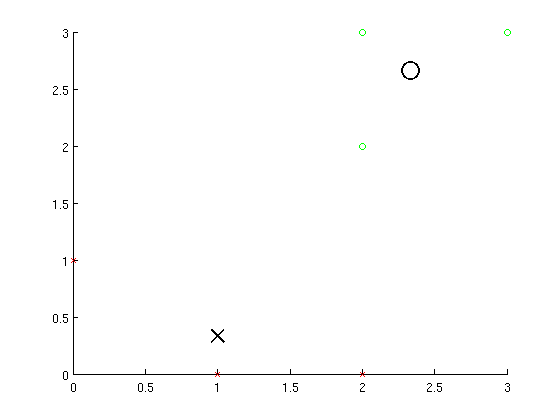
\includegraphics[width=1\linewidth]{../img/data7b11.png}
    \caption{$b = 1.1$}
  \end{minipage}
  \begin{minipage}[b]{0.5\linewidth}
    \centering
    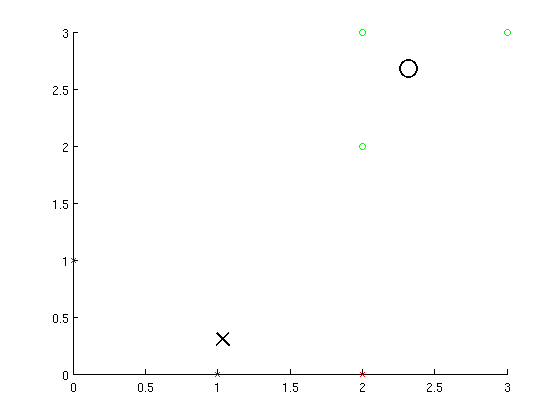
\includegraphics[width=1\linewidth]{../img/data7b2.png}
    \caption{$b = 2$}	
  \end{minipage}
\end{figure}
\begin{figure}[h]
    \centering
    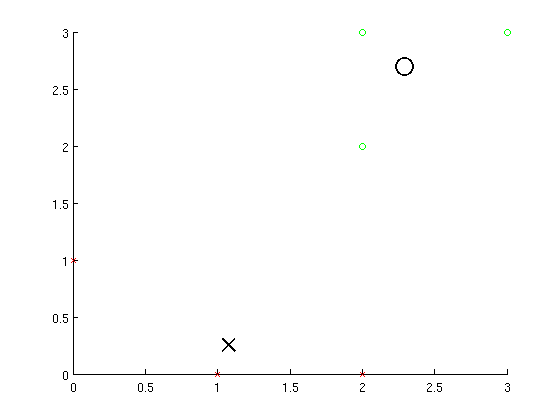
\includegraphics[width=0.5\linewidth]{../img/data7b3.png}
    \caption{$b = 3$}
\end{figure}

\FloatBarrier
\subsection*{Versuch 2}
Datensatz aus Aufgabe 7, Fuzzifier $b = 2$, Toleranz $\epsilon$ variert zwischen $1*e^{-2}$ und $1*e^{-10}$:
\begin{figure}[h]
  \begin{minipage}[b]{0.5\linewidth}
    \centering
    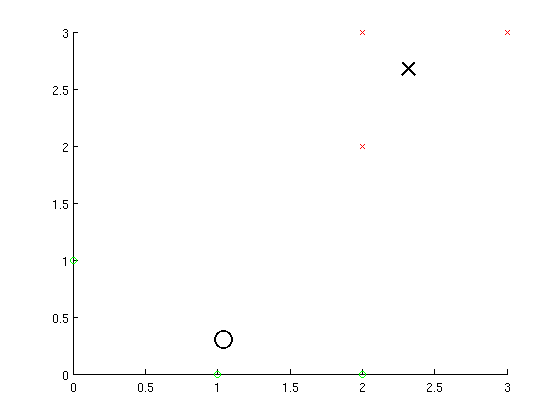
\includegraphics[width=1\linewidth]{../img/data7b2e2.png}
    \caption{$\epsilon = 1*e^{-2}$}
  \end{minipage}
  \begin{minipage}[b]{0.5\linewidth}
    \centering
    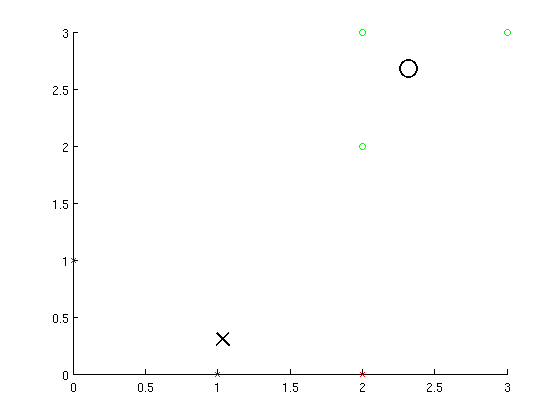
\includegraphics[width=1\linewidth]{../img/data7b2e5.png}
    \caption{$\epsilon = 1*e^{-5}$}	
  \end{minipage}
\end{figure}
\begin{figure}[h]
    \centering
    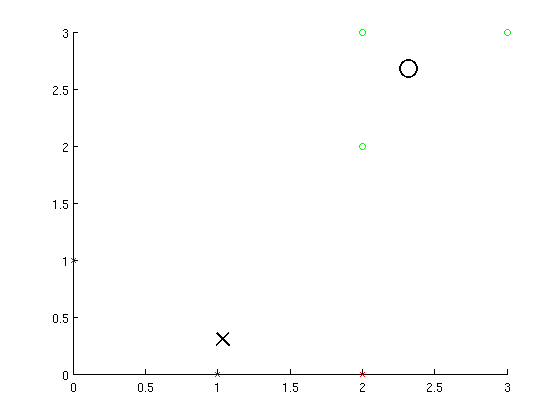
\includegraphics[width=0.5\linewidth]{../img/data7b2e10.png}
    \caption{$\epsilon = 1*e^{-10}$}
\end{figure}

\FloatBarrier
\subsection*{Versuch 3}
Datensatz aus Aufgabe 8, Toleranz $\epsilon = 1*e^{-5}$, Clusteranzahl $k = 2$, Fuzzifier $b$ variert zwischen 1.1 und 3:
\begin{figure}[h]
  \begin{minipage}[b]{0.5\linewidth}
    \centering
    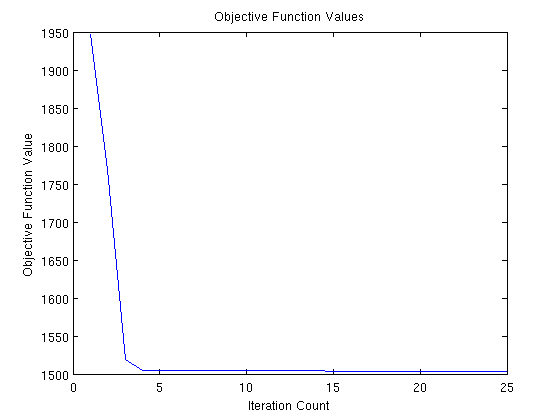
\includegraphics[width=1\linewidth]{../img/data8b11e5c2.png}
    \caption{$b = 1.1$}
  \end{minipage}
  \begin{minipage}[b]{0.5\linewidth}
    \centering
    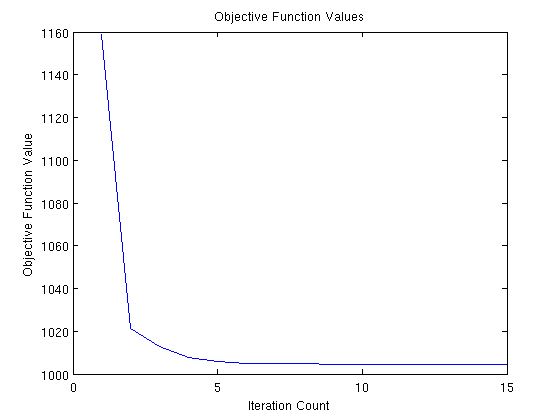
\includegraphics[width=1\linewidth]{../img/data8b2e5c2.png}
    \caption{$b = 2$}	
  \end{minipage}
\end{figure}
\begin{figure}[h]
    \centering
    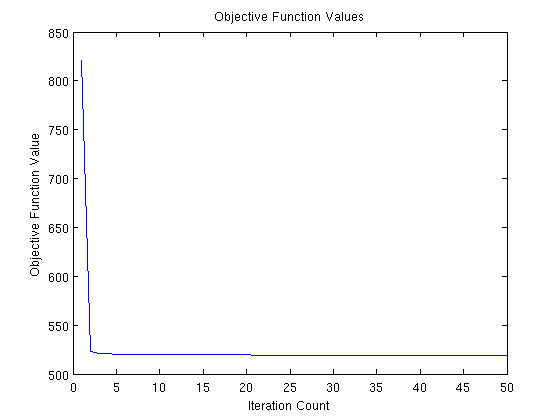
\includegraphics[width=0.5\linewidth]{../img/data8b3e5c2.png}
    \caption{$b = 3$}
\end{figure}

\FloatBarrier
\subsection*{Versuch 4}
Datensatz aus Aufgabe 8, Toleranz $\epsilon = 1*e^{-5}$, Fuzzifier $b = 2$, Clusteranzahl $k$ variert zwischen 2 und 5:
\begin{figure}[h]
  \begin{minipage}[b]{0.5\linewidth}
    \centering
    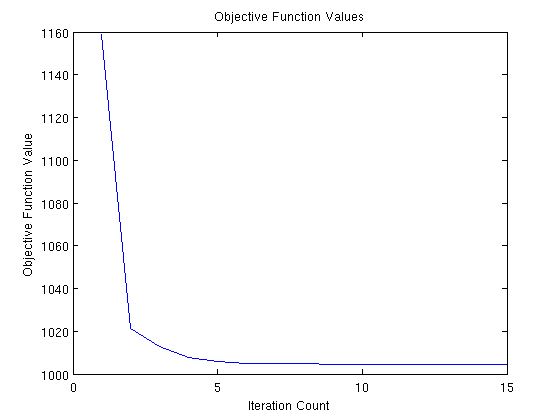
\includegraphics[width=1\linewidth]{../img/data8b2e5c2.png}
    \caption{$k = 2$}
  \end{minipage}
  \begin{minipage}[b]{0.5\linewidth}
    \centering
    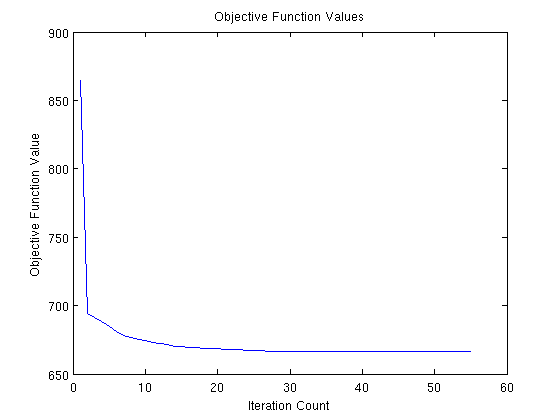
\includegraphics[width=1\linewidth]{../img/data8b2e5c3.png}
    \caption{$k = 3$}	
  \end{minipage}
\end{figure}
\begin{figure}[h]
    \centering
    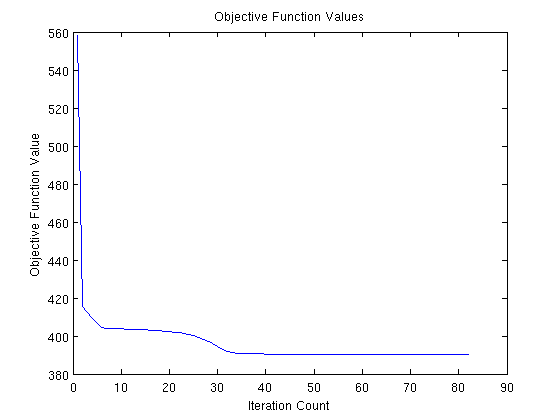
\includegraphics[width=0.5\linewidth]{../img/data8b2e5c5.png}
    \caption{$k = 5$}
\end{figure}
\end{document}
